\section{Implémentation}

\subsection{Hiérarchie complète}
\label{sec:sig-hierarchy}

La figure \ref{sec:sig-hierarchy} présente la hiérarchie formée par les différentes classes de signaux. Cette section aborde plus en détails les spécificités de chacune d'elles.

\begin{figure}[h]
	\centering
	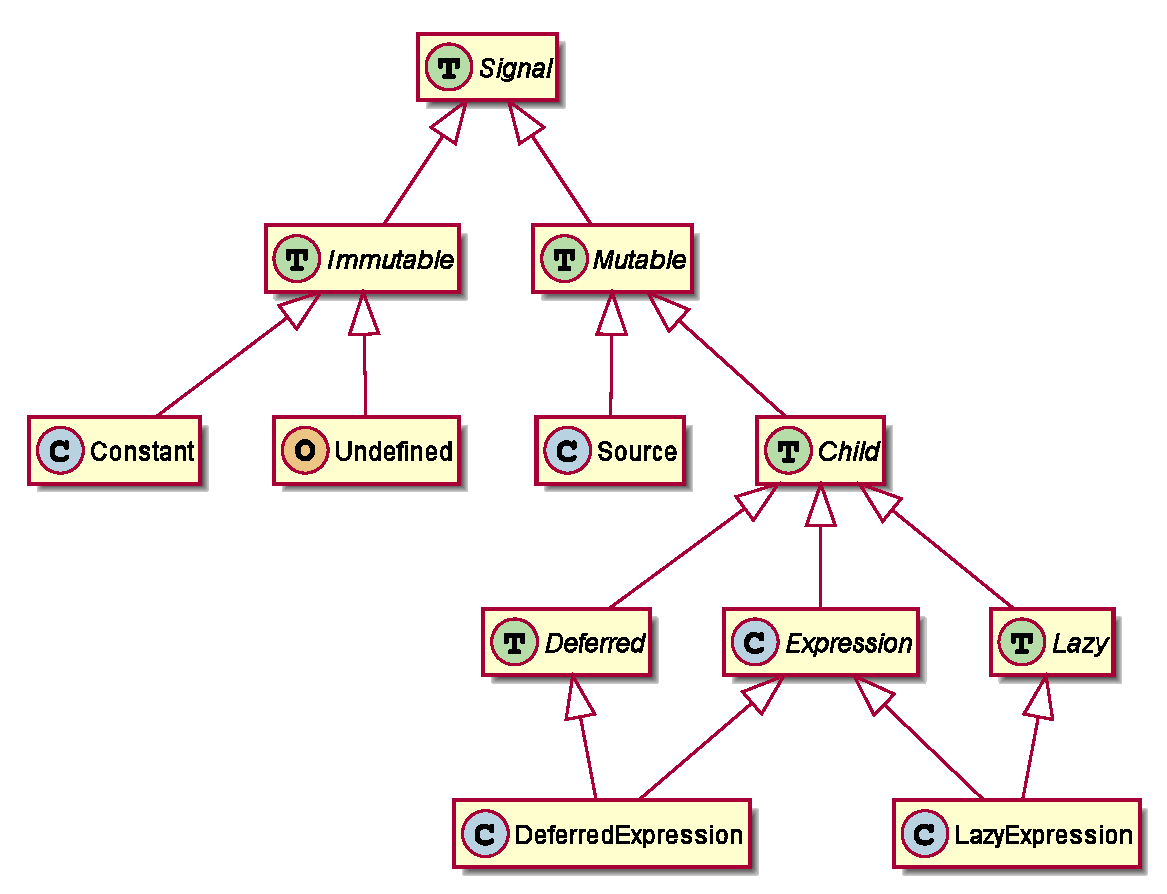
\includegraphics[width=10cm]{img/sig_hierarchy.eps}
	\caption{Hiérarchie des signaux}
	\label{fig:sig-hierarchy}
\end{figure}

L'implémentation des signaux est organisée sur la base du raffinement successif de la sémantique d'un signal. Chaque niveau laisse généralement un point de sa sémantique indéfini, sous la forme d'une méthode abstraite à implémenter par les sous-classes.

\begin{itemize}
	\item \texttt{Signal}: la vue la plus générale d'un signal, ce trait définit les méthodes de transformation et d'accès à l'état du signal. La fonction \texttt{def option: T} est indéfinie et doit retourner l'état courante du signal.
	\item \texttt{Immutable}: redéfinit \texttt{option} en \texttt{val} puisque l'état est immutable, mais laisse la valeur abstraite.
	\item \texttt{Constant}: définit \texttt{val option = Some(value)}
	\item \texttt{Undefined}: définit \texttt{val option = None}
	\item \texttt{Mutable}: déclare la méthode abstraite \texttt{def current: Option[T]}, représentant également l'état du signal mais dont le nom indique clairement la mutabilité du signal.
	
	Définit la méthode \texttt{option} en se basant sur \texttt{current} mais y ajoute la détection automatique des signaux enfants. De cette façon, toutes les méthodes de \texttt{Signal}, en utilisant directement ou indirectement \texttt{option}, obtiennent également les mécanismes de détection.
	
	\item \texttt{Source}: définit une variable interne pour stocker l'état de la source, implémente \texttt{current} sur la base de cette variable.
	
	Ajoute également les opérations de mutation explicites.
	
	\item \texttt{Child}: déclare la méthode abstraite \texttt{def generate: Option[T]}, appelée lorsque l'état du signal doit être calculé. Implémente \texttt{current} sur la base de \texttt{generate} et y ajoute le mécanisme de \emph{memoization}.
	
	Définit la méthode \texttt{def invalidate(): Unit} qui permet d'effacer l'état mémorisé du signal et d'invalider récursivement tous les signaux enfants. Cette méthode est en principe appelée par \texttt{Mutable}.
	
	\item \texttt{Lazy}: trait \emph{marqueur}, l'implémentation de \texttt{Child} utilise déjà la sémantique \emph{lazy} par défaut. Il n'y a donc rien à modifier.
	
	\item \texttt{Deferred}: surcharge la méthode \texttt{invalidate} définie par \texttt{Child} en insérant le signal dans la queue du contexte de mutation courant. De cette façon, ce signal sera recalculé de façon différée à la fermeture du contexte de mutation.
	
	\item \texttt{Expression}: implémente \texttt{generate} sur la base de l'expression passée en paramètre.
	
	\item \texttt{LazyExpr}: combine \texttt{Expression} avec \texttt{Lazy}
	\item \texttt{DeferredExpr}: combine \texttt{Expression} avec \texttt{Deferred}
\end{itemize}

Les classes \texttt{LazyExpr} et \texttt{DeferredExpr} sont privées. S'il est nécessaire dans le code utilisateur de déterminer la sémantique d'une expression, un \emph{pattern matching} sur les traits \texttt{Lazy} et \texttt{Deferred} peut être effectué. Il est également possible de tester si un signal est une expression constante avec l'opérateur \texttt{with}, sous la forme: \code{case e: Expression with Lazy}.

\subsection{Détection automatique des dépendances}

La détection automatique des dépendances des signaux et observateurs joue un rôle essentiel dans l'implémentation des signaux. Même à l'intérieur de la bibliothèque, aucune dépendance n'est déclarée explicitement et le détection automatique est utilisée.

L'élément clé de ce mécanisme est la classe \texttt{x.s.t.TracingContext}. Un contexte de traçage est un mécanisme très similaire à celui du contexte de mutation (§ \ref{sec:sig-mut-context}). Les deux sont construits sur la base du mécanisme de \texttt{DynamicVariable} présent dans la bibliothèque standard Scala.

Une opération de traçage est effectuée par un appel à la méthode
\begin{center}
	\code{def TracingContext.trace[T](expr: => T): (T, List[Mutable[_]])}
\end{center}
prenant en paramètre une expression arbitraire qui sera évaluée. La méthode retourne un couple de valeurs, dont le premier membre est le résultat de l'évaluation de l'expression et le second la liste de tous les signaux qui ont été accédés lors de cette évaluation.

Il convient de noter que seuls des signaux de type \texttt{Mutable[\_]} sont retournés. En effet, cette liste à pour but d'énumérer les dépendances de l'expression évaluée et ainsi permettre la mise en place des notifications de mises à jour. Un signal immutable ne changeant par définition jamais, il n'y a pas d'intérêt à le considérer comme une dépendance de l'expression.

La classe \texttt{DynamicVariable} est conçue pour représenter une variable dont la valeur et déterminée par portée dynamique plutôt que portée lexicale. C'est-à-dire que la valeur de la variable est déterminée dynamiquement selon la pile d'appel à l'exécution plutôt que par la structure du code source.

En pratique, il n'existe pas de portée dynamique en Scala, le concept est donc émulé en utilisant une pile locale au thread courant afin de stocker la valeur de la variable. La méthode
\begin{center}
	\code{def DynamicVariable[T].withValue[U](v: T)(expr: => U): U}
\end{center}
permet l'exécution d'un bloc de code arbitraire durant laquelle la méthode \texttt{DynamicVariable.value} retournera la valeur passée en paramètre. Chaque invocation de la méthode \texttt{withValue} ajoute un nouvel étage à la pile qui sera dépilé une fois l'évaluation terminée.

Dans le cas de \texttt{TracingContext}, un nouveau contexte est créé lors de l'appel à la méthode \texttt{trace} et placé dans une variable \texttt{DynamicVariable}. La seconde partie du système est implémentée dans la classe \texttt{Mutable}. Comme indiqué dans le détail de la hiérarchie des signaux (§ \ref{sec:sig-hierarchy}), cette classe implémente la méthode \emph{option} de \texttt{Signal} en y ajoutant le mécanisme de détection des dépendances.

Plus spécifiquement, chaque invocation de la méthode \texttt{option} d'un signal \texttt{Mutable} va appeler la méthode interne \texttt{TracingContext.record} afin d'enregistrer l'accès au signal dans le contexte courant. Déterminer le \emph{contexte courant} consiste en un simple accès à la variable \texttt{DynamicVariable} mentionnée précédemment.

Contrairement aux contextes de mutations, l'imbrication des contextes de traçage est significative. L'accès à un signal ne sera en effet enregistré que dans le contexte le plus récent, au sommet de la pile. Ceci découle de l'utilisation de contextes de traçage, en interne, par les signaux expression. 

L'objectif final est de limiter la liste des signaux retournés par la méthode \texttt{trace} aux dépendances directes de l'expression évaluée. Il n'est en effet pas intéressant de récupérer les dépendances \emph{transitives} d'un signal puisque les notification de mises à jour sont propagées récursivement jusqu'aux feuilles du graphe.

La figure \ref{fig:sig-nested-tracing} illustre une situation d'imbrication des contextes de traçage. L'évaluation du signal \emph{E} crée un nouveau contexte qui sera utilisé pour déterminer ses dépendances. Lors de l'évaluation du signal \emph{C}, un nouveau contexte est créé pour déterminer les dépendances de ce signal. Les signaux \emph{B} et \emph{A} forment ainsi des dépendances \emph{transitives} de \emph{E} et ne seront pas retournées dans la liste de signaux accédés par le signal \emph{E}, celle-ci se limitant aux signaux \emph{D} et \emph{C}.

\begin{figure}[h]
	\centering
	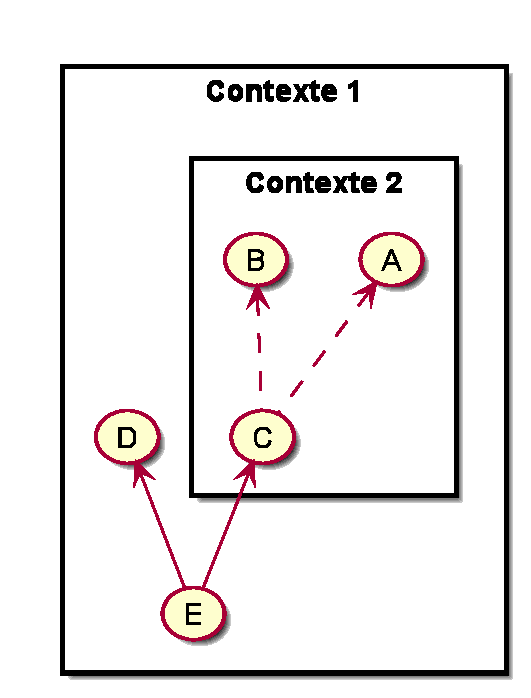
\includegraphics[width=5cm]{img/signals_nested_tracing.eps}
	\caption{Imbrication des contextes de traçage}
	\label{fig:sig-nested-tracing}
\end{figure}

Cette approche est une alternative à l'utilisation de paramètres implicites, tels qu'utilisés par la bibliothèque \emph{Scala.rx} \cite{scala.rx}. Les variables dynamiques forment un canal indépendant pour déterminer les relations de dépendance entre signaux et observateurs. Il n'est alors plus nécessaire de recourir à des macros compilateur pour transformer automatiquement l'expression fournie par l'utilisateur en fonction anonyme.

En contre-partie, la détection de dépendances est maintenant liée à la structure de la pile d'appels lors de l'accès aux signaux, ce qui implique une exécution synchrone des opérations. Les structures \emph{lazy} ou \emph{asynchrones} sont donc particulièrement problématiques puisqu'elles ne conservent pas la variable dynamique qui sera perdue dès la retour de l'appel synchrone. Dans un environnement \emph{single-threaded} tel que JavaScript, ceci n'est cependant pas un problème.

\subsection{Implémentation des opérateurs de transformation}

Lors de l'implémentation des opérateurs de transformation, deux approches ont été envisagées:
\begin{enumerate}
	\item Implémentation d'une sous-classe de \texttt{Signal} par transformation, par exemple des classes \texttt{Map}, \texttt{Fold}, etc. Cette approche est par exemple utilisée par la bibliothèque \emph{Bindings.scala} \cite{binding.scala}.
	\item Réutiliser le mécanisme des signaux expressions.
\end{enumerate}

La seconde approche a été choisie sur la base de la réutilisation de l'ensemble des mécanismes développés pour les signaux expression. Le seul élément à considérer est alors l'implémentation concrète de la transformation. Les détails annexes, tels que la sémantique d'évaluation ou la gestion des dépendances est obtenue de façon automatique.

Par exemple, la transformation \texttt{map} est déclarée simplement par
\begin{center}
	\code{def map[U](f: T => U): Signal[U] =}\\
	\code{Signal.define(option.map(f)) }
\end{center}
Ici, \texttt{option} fait référence à la méthode \texttt{Signal.option}. Le type de signal retourné par une transformation dépend du type de signal sur lequel elle est invoquée. Appliquer une transformation \texttt{map} sur un signal \texttt{Constant} retourne un nouveau signal \texttt{Constant}. Ceci résulte du fait que, lors du calcul de l'expression de définition de la transformation, aucun signal \texttt{Mutable} n'a été accédé. Le constructeur \texttt{Signal.define} retourne alors un signal de type \texttt{Constant} ce qui correspond au comportement attendu de la transformation.

Dans une version antérieure de l'implémentation des signaux, ces transformations étaient déclarées de façon abstraite dans l'interface \texttt{Signal} puis implémentées indépendamment dans les sous-classes \texttt{Mutable} et \texttt{Immutable}. Avec l'amélioration du constructeur \texttt{Signal.define}, prenant en compte les signaux accédés lors de la définition d'un nouveau signal, cette complexité a pu être éliminée et l'ensemble des signaux, mutables comme immutables, partagent maintenant une définition unique dans la classe parente \texttt{Signal}.

Un effet secondaire supplémentaire de cette implémentation est le support de fonctions de transformation impures. Référencer la valeur d'autres signaux dans une fonction passée aux opérateurs produira le résultat attendu. La figure \ref{fig:sig-map-pureness} illustre une telle situation où un même signal \texttt{Constant} est transformé en un nouveau signal \texttt{Constant} ou une \texttt{Expression} selon la pureté de la fonction passée en paramètre. Le support de ce style, bien que d'une élégance discutable, permet de réduire le risque de surprendre un utilisateur qui s'attendrait à pouvoir se servir de telles constructions.

\begin{figure}
	\begin{lstlisting}
val a: Constant[Int] = Constant(2)
val b: Signal[Int] = ...

val c = a.map(_ * 2)
// `c` est un signal `Constant[Int]`

val d = a.map(_ * b.value)
// `d` est un signal `Expression[Int]`
	\end{lstlisting}
	\caption{Exemple de transformation d'un signal constant en utilisant des fonctions pures ou impures}
	\label{fig:sig-map-pureness}
\end{figure}

\subsection{Modèle push, pull ou hybride}

Deux modes de fonctionnement sont généralement décrits pour des systèmes fonctionnels-réactifs: \emph{push} et \emph{pull}.

L'approche \emph{push} se base sur les changements apportés aux signaux sources pour recalculer tous les signaux enfants qui en dépendent. Dans l'approche \emph{pull}, c'est l'accès aux signaux enfants qui provoque le calcul des valeurs intermédiaires jusqu'aux signaux sources. Dans les deux cas, des opérations potentiellement inutiles ou redondantes sont effectuées.

L'approche mixte \emph{push-pull} se base sur une approche principalement \emph{pull} où l'accès à l'état d'un signal déclenche son évaluation, à laquelle vient s'ajouter un mécanisme de \emph{memoization} qui maintient l'état courant du signal après son calcul. L'invalidation de ces caches se fait ensuite selon une approche \emph{push}: un changement d'état des signaux sources est notifié à toutes les dépendances de façon récursive.

Dans le cadre de ce projet, l'approche \emph{pull} était tout simplement inutilisable. Lors de l'implémentation d'une interface utilisateur, les notifications de mises à jour proviennent des racines du graphe de signaux. L'interface ne connaît \emph{a priori} pas les moments opportuns à l'exécution d'un \emph{pull} pour se mettre à jour. L'approche \emph{push} est déjà plus adaptée, mais impose une mise à jour complète du graphe à chaque changement.

L'architecture proposée de l'application associe un graphe de signaux, représentant l'ensemble des données disponibles, avec un ensemble d'observateurs, correspondant aux données actuellement utilisées par l'interface. Il est courant qu'une partie de ce graphe soit inutilisée dans l'état courant de l'interface. Lorsque l'utilisateur navigue dans l'application, les observateurs des données qui ne sont plus visibles sont retirés tandis que de nouveaux sont attachés sur les données qui apparaissent à l'écran. Ainsi, les sections du graphe considérées actives changent dynamiquement en fonction des actions effectuées par l'utilisateur.

Le modèle hybride permet aux sections actives du graphe, celles dont les feuilles disposent d'observateurs, de se comporter effectivement de façon \emph{push} en étant recalculées dès lors que les données sources sont modifiées. À l'inverse, les sections inactives du graphe se comportent de façon \emph{pull}, n'étant pas recalculées inutilement tant qu'un observateur n'y aura pas été attaché ou leur état courant accédé de façon explicite.
